% Using Free and Open Source Solutions in Geospatial Science Education
% This work by Vaclav Petras is licensed under
% a Creative Commons Attribution-ShareAlike 4.0 International License.

\documentclass[xcolor={dvipsnames,usenames},beamer,aspectratio=169]{beamer}
% ,handout,notes=show

\makeatletter
\def\beamer@framenotesbegin{% at beginning of slide
  \gdef\beamer@noteitems{}%
  \gdef\beamer@notes{{}}% used to be totally empty.
}
\makeatother

\usepackage{textcomp}
\usepackage[utf8]{inputenc}
\usepackage[american]{babel}
\usepackage{graphicx}
\usepackage{url}

\usepackage{tikz}
\usetikzlibrary{arrows,shapes,spy,calc}

\tikzstyle{every picture}+=[remember picture]
\tikzstyle{na} = [baseline=-.5ex]

% frames have to be fragile
\newif\ifnotes
% \input{tmpnotessettings}
% \notestrue


\ifnotes
\setbeamertemplate{note page}[plain]
% \setbeamertemplate{note page}[compress]
\setbeamerfont{note page}{size=\large}
% \setbeameroption{show only notes}
\setbeameroption{show notes}
\usepackage{pgfpages}
\pgfpagesuselayout{2 on 1}[a4paper,border shrink=5mm]%
\else
%\setbeameroption{hide notes}
\fi
%\notesfalse

\usepackage[absolute,overlay]{textpos}

\usepackage{listings}


% \usetheme{Warsaw}
\usetheme{Madrid}
% \usetheme{Frankfurt}
% \useoutertheme{infolines}
\usecolortheme[named=MidnightBlue]{structure}
% \usecolortheme[named=PineGreen]{structure}
\setbeamertemplate{navigation symbols}{}

\setbeamertemplate{itemize items}[default]
\setbeamertemplate{enumerate items}[default]
% \useinnertheme{rectangles}
\setbeamertemplate{blocks}[default]


%%%%%%%%%%%%%%%%%%%%%%%%%%%%%%%%%%%%%%%%%%%%%%%%%%%%%%%%%%%%%%%%%%%%
%%%%%%%%%%%%%%%%%%%%%%%%%%%%%%%%%%%%%%%%%%%%%%%%%%%%%%%%%%%%%%%%%%%%

% \newcommand{\n}[1]{$^{\color{gray}{\mbox{\tiny#1}}}$}
\newcommand{\n}[1]{$^{\textcolor{gray}{\mbox{\tiny{#1}}}}$}

%%%%%%%%%%%%%%%%%%%%%%%%%%%%%%%%%%%%%%%%%%%%%%%%%%%%%%%%%%%%%%%%%%%%%%%%%%%%%%%
\newcommand{\gmodule}[1]{\href{http://grass.osgeo.org/grass71/manuals/#1.html}{\emph{#1}}}
\newcommand{\asixmodule}[1]{\emph{#1}}
\newcommand{\asevenmodule}[1]{\emph{#1}}
\newcommand{\module}[1]{\emph{#1}}
\newcommand{\grasslink}{\href{http://grass.osgeo.org/}{GRASS GIS}}

%%%%%%%%%%%%%%%%%%%%%%%%%%%%%%%%%%%%%%%%%%%%%%%%%%%%%%%%%%%%%%%%%%%%
%%%%%%%%%%%%%%%%%%%%%%%%%%%%%%%%%%%%%%%%%%%%%%%%%%%%%%%%%%%%%%%%%%%%

\title%[Processing of point clouds]
{New lidar processing functionality in GRASS GIS 7.1}
\subtitle{webinar for USFWS Remote Sensing group}
%\pdforstring{}{}

\author[Vaclav Petras]
{Vaclav Petras (Vashek)%\n{1}\\
%{\scriptsize
%Anna Petrasova\n{1},
%\mbox{
%Helena Mitasova\n{1}
%}
%}
}

\institute[NC State University]
{%
%$^1$%
North Carolina State University, Center for Geospatial Analytics \\
\bigskip
\includegraphics[width=0.3\textwidth]{logos/ncstate}
}

\date{February 22, 2016}

\setbeamercovered{transparent}

\hypersetup{%
 pdfauthor={Vaclav Petras},%
 pdfsubject={UAV/lidar data analytics course project presentation},%
 pdfkeywords={UAV} {UAS} {point clouds} {lidar}
   {v.in.lidar} {r.in.lidar} {v.decimate} {v.out.lidar} {libLAS}
   {geospatial modeling} {GRASS GIS}
   {free software} {open source} {open science}
}

\usepackage{tipa}
\newcommand{\pron}[2]{#1 [#2]}


\newcommand{\beginbackup}{
  \newcounter{framenumbervorappendix}
  \setcounter{framenumbervorappendix}{\value{framenumber}}
}
\newcommand{\backupend}{
  \addtocounter{framenumbervorappendix}{-\value{framenumber}}
  \addtocounter{framenumber}{\value{framenumbervorappendix}}
}


%%%%%%%%%%%%%%%%%%%%%%%%%%%%%%%%%%%%%%%%%%%%%%%%%%%%%%%%%%%%%%%%%%%%
% when images are placed in these directories, we don't have to specify the directory
% just the filename
\graphicspath{{img/}{figures/}{images/}}


%%%%%%%%%%%%%%%%%%%%%%%%%%%%%%%%%%%%%%%%%%%%%%%%%%%%%%%%%%%%%%%%%%%%
%%%%%%%%%%%%%%%%%%%%%%%%%%%%%%%%%%%%%%%%%%%%%%%%%%%%%%%%%%%%%%%%%%%%
%%%%%%%%%%%%%%%%%%%%%%%%%%%%%%%%%%%%%%%%%%%%%%%%%%%%%%%%%%%%%%%%%%%%
%%%%%%%%%%%%%%%%%%%%%%%%%%%%%%%%%%%%%%%%%%%%%%%%%%%%%%%%%%%%%%%%%%%%
\begin{document}

\newcommand{\logowidth}{1.0em}
\newcommand{\logospace}{\hspace{0.2em}}
\newcommand{\includecclogo}[1]{\includegraphics[width=\logowidth]{./images/logos/#1}}

%%%%%%%%%%%%%%%%%%%%%%%%%%%%%%%%%%%%%%%%%%%%%%%%%%%%%%%%%%%%%%%%%%%%
\frame{
\titlepage
\begin{center}
\vspace{-3ex}
\href{http://creativecommons.org/licenses/by-sa/4.0/}{
\includecclogo{cc}
\logospace
\includecclogo{by}
\logospace
\includecclogo{sa}
}
\end{center}
}


%%%%%%%%%%%%%%%%%%%%%%%%%%%%%%%%%%%%%%%%%%%%%%%%%%%%%%%%%%%%%%%%%%%%%
\begin{frame}{GRASS GIS architecture}

\begin{columns}
\begin{column}{0.4\textwidth}

\begin{block}{Functionality}
 \begin{itemize}
  \item split to modules
  \item independent of GUI
  \item integrated to GUI
  \item unified access to all functions
\end{itemize}
\end{block}

\end{column}
\begin{column}{0.4\textwidth}

\begin{center}
  \includegraphics[width=0.5\textwidth]{logos/grass_gis}
\end{center}

\end{column}
\end{columns}

\end{frame}

%%%%%%%%%%%%%%%%%%%%%%%%%%%%%%%%%%%%%%%%%%%%%%%%%%%%%%%%%%%%%%%%%%%%%
\begin{frame}{GRASS GIS architecture}

\begin{columns}
\begin{column}{0.4\textwidth}

\begin{block}{Modules}
 \begin{itemize}
%\begin{itemize}
  \item GUI just one of the modules: g.gui, g.gui.gmodeler, g.gui.animation
  \item all important ones available in the basic installation $>$500
  \item extra and experimental modules in addons repository {\raise.17ex\hbox{$\scriptstyle\sim$}}250
\end{itemize}

% cd trunk/dist.x86_64-pc-linux-gnu
% find scripts bin -executable -type f | wc

% cd addons/grass7
% find . -name "*.html" | wc

\end{block}

\end{column}
\begin{column}{0.45\textwidth}

\begin{center}
  \includegraphics[width=\textwidth]{grass/count_and_modules}
\end{center}

\end{column}
\end{columns}

\end{frame}


%%%%%%%%%%%%%%%%%%%%%%%%%%%%%%%%%%%%%%%%%%%%%%%%%%%%%%%%%%%%%%%%%%%%%
\begin{frame}{GRASS GIS architecture}

\begin{columns}
\begin{column}{0.4\textwidth}

\begin{block}{General modules}
g.list, g.remove, g.copy
\end{block}

\begin{block}{Raster modules}
r.contour, r.watershed, r.li.patchdensity
\end{block}

\begin{block}{Vector modules}
v.generalize, v.db.select, v.net.salesman
\end{block}

\end{column}
\begin{column}{0.45\textwidth}

\begin{center}
  \includegraphics[width=\textwidth]{grass/basins}
\end{center}

\end{column}
\end{columns}

% \begin{block}{Modules}
% \begin{tabular}{lll}
% group & prefix & examples \\\hline
% general & g. & g.list, g.remove, g.copy \\
% raster & r. & r.contour, r.watershed, r.li.patchdensity \\
% vector & v. & v.generalize, v.db.select, v.net.salesman \\
% 3D raster & r3. & r3.mapcalc, r3.univar, r3.gwflow \\
% imagery & i. & i.maxlik, i.pca, i.segment \\
% temporal & t. & t.rast.aggregate, t.rast.accdetect, t.vect.univar \\
% \end{tabular}
% \end{block}

\end{frame}

%%%%%%%%%%%%%%%%%%%%%%%%%%%%%%%%%%%%%%%%%%%%%%%%%%%%%%%%%%%%%%%%%%%%%
\begin{frame}{GRASS GIS architecture}

\begin{columns}
\begin{column}{0.4\textwidth}

\begin{block}{3D raster modules}
r3.mapcalc, r3.univar, r3.gwflow
\end{block}

\begin{block}{Imagery modules}
i.maxlik, i.pca, i.segment
\end{block}

\begin{block}{Temporal modules}
t.rast.aggregate, t.rast.accdetect, t.vect.univar
\end{block}

\end{column}
\begin{column}{0.45\textwidth}

\begin{center}
  \includegraphics[width=\textwidth]{grass/segment_on_counts}
\end{center}

% method=n class=2
% method=n class=1
% i.group
% i.segement 0.75

\end{column}
\end{columns}

\end{frame}

%%%%%%%%%%%%%%%%%%%%%%%%%%%%%%%%%%%%%%%%%%%%%%%%%%%%%%%%%%%%%%%%%%%%%
% \begin{frame}{GRASS GIS architecture}

% \begin{block}{Modules}
% \begin{tabular}{lll}
% group & prefix & examples \\\hline
% general & g. & g.list, g.remove, g.copy \\
% raster & r. & r.contour, r.watershed, r.li.patchdensity \\
% vector & v. & v.generalize, v.db.select, v.net.salesman \\
% 3D raster & r3. & r3.mapcalc, r3.univar, r3.gwflow \\
% imagery & i. & i.maxlik, i.pca, i.segment \\
% temporal & t. & t.rast.aggregate, t.rast.accdetect, t.vect.univar \\
% \end{tabular}
% \end{block}

% \end{frame}

%%%%%%%%%%%%%%%%%%%%%%%%%%%%%%%%%%%%%%%%%%%%%%%%%%%%%%%%%%%%%%%%%%%%%
\begin{frame}{GRASS GIS architecture}

\begin{block}{Data}
 \begin{itemize}
  \item unified format and projection, vector and temporal topology
    \begin{itemize}
      \item solve data inconsistencies at the beginning, then focus only on the analysis
    \end{itemize}
  \item computation region (extent and resolution) independent of data
    \begin{itemize}
      \item all raster operations respect the region for inputs and outputs
    \end{itemize}
  \item exceptions: lidar data processing
    \begin{itemize}
      \item large point clouds
      \item input for processing in point cloud formats
    \end{itemize}
 \end{itemize}
\end{block}

\end{frame}

%%%%%%%%%%%%%%%%%%%%%%%%%%%%%%%%%%%%%%%%%%%%%%%%%%%%%%%%%%%%%%%%%%%%%
\begin{frame}{Scripting}

\begin{block}{Python}
 \begin{itemize}
  \item simple scripting but also advanced programming
  \item \texttt{run\_command('r.in.lidar', file=files.txt, output='surface', method='max', class\_filter=[1, 2], flags='e')}
 \end{itemize}
\end{block}

\begin{block}{Bash (shell)}
 \begin{itemize}
  \item simple syntax, easy to work with files, for simple task
  \item native to Linux, possible to use on MS Windows (e.g. MSYS)
  \item \texttt{r.in.lidar -e file=files.txt output=max method=max class\_filter=1,2}
 \end{itemize}
\end{block}

\begin{small}
also R: \texttt{execGRASS("r.in.lidar", file="files.txt", output="max", method="max", ...)}
\end{small}

\end{frame}

%%%%%%%%%%%%%%%%%%%%%%%%%%%%%%%%%%%%%%%%%%%%%%%%%%%%%%%%%%%%%%%%%%%%%
\begin{frame}{GUI and scripting interface convergence}

\centering
\includegraphics[width=\textwidth]{grass/grass_cmd_gui}%

\end{frame}

%%%%%%%%%%%%%%%%%%%%%%%%%%%%%%%%%%%%%%%%%%%%%%%%%%%%%%%%%%%%%%%%%%%%%
\begin{frame}{Typical lidar workflow}

\begin{columns}
\begin{column}{0.5\textwidth}

% \begin{block}{Explore the data with \gmodule{r.in.lidar}}
Explore the data with \gmodule{r.in.lidar}
 \begin{itemize}
  \item import extent based on input data (\texttt{-e}~flag)
  \item resolution set to high number (coarse, \texttt{resolution=10})
  \item counting number of points per cell (\texttt{method=n})
  \item trying different class and return filters (\texttt{class\_filter}, \texttt{return\_filter})
  \item decide on computational region extent and resolution (\texttt{g.region})
 \end{itemize}
% \end{block}

\end{column}
\begin{column}{0.45\textwidth}

\begin{center}
  \includegraphics[width=0.75\textwidth]{grass/rinlidar_region}

  \footnotesize
  r.in.lidar, 578 million points in 90 files to 1882 $\times$ 1651 cells using 50MiB in 2 min

% time r.in.lidar file=list_las_files.txt -e method=n output=count res=5 --o
% 578628031 points from 90 files found in region
%
% r.in.lidar: 2m14.852s 50MiB
% r.info map=count@all -g
% north=3886000
% south=3876590
% east=281705
% west=273450
% nsres=5
% ewres=5
% rows=1882
% cols=1651
% cells=3107182
% datatype=CELL
% ncats=0
%
% r.in.lidar: 2m25.048s 1.2GiB
% r.info map=count_2@all -g
% north=3886000
% south=3876590.5
% east=281700.5
% west=273452
% nsres=0.5
% ewres=0.5
% rows=18819
% cols=16497
% cells=310457043
% datatype=CELL
% ncats=0

% g.region rast=count_2@all
% r.univar map=count_2@all -e
% 30 sec

\end{center}

\end{column}
\end{columns}

\end{frame}


%%%%%%%%%%%%%%%%%%%%%%%%%%%%%%%%%%%%%%%%%%%%%%%%%%%%%%%%%%%%%%%%%%%%%
\begin{frame}{Typical lidar workflow}


\begin{columns}
\begin{column}{0.5\textwidth}

Analyze with \gmodule{r.in.lidar}
 \begin{itemize}
  \item statistics of point counts, height and intensity
  \item using different resolutions
 \end{itemize}

Create surface with \gmodule{v.in.lidar} and interpolation
 \begin{itemize}
  \item import selected points (spatial extent, classes and returns)
  \item interpolate surface (\gmodule{v.surf.rst}, \gmodule{v.surf.bspline}, \gmodule{v.surf.idw})
  \item smooth surface without NULL cells
  \end{itemize}

Continue analysis using standard GRASS GIS tools
% rasterize soon (if you can)

\end{column}
\begin{column}{0.45\textwidth}

\begin{center}
  \includegraphics[width=0.8\textwidth]{grass/range_on_smooth_max_larger}

  \footnotesize
  r.in.lidar and r.neighbors, range smoothed maximum surface,
  550927433 points from 90 files to 8076 x 7223 cells
  using 480MiB in 4 min
  % 1 + 37.262/60 + 1 + 47.132/60 + 11./60
\end{center}

% g.region -p
% north:      3885316.5
% south:      3877241.5
% west:       273832
% east:       281053
% nsres:      0.5
% ewres:      0.5
% rows:       16150
% cols:       14442
% cells:      233238300

% r.in.lidar max
% 550927433 points from 90 files found in region
% 920MiB
% 1m39.372s

% g.region -p
% north:      3885316.5
% south:      3877241.25
% west:       273831.75
% east:       281053.5
% nsres:      0.75
% ewres:      0.75
% rows:       10767
% cols:       9629
% cells:      103675443

% r.in.lidar max
% 550927433 points from 90 files found in region
% 430MiB
% 1m38.932s


% g.region -p
% north:      3885317
% south:      3877241
% west:       273831
% east:       281054
% nsres:      1
% ewres:      1
% rows:       8076
% cols:       7223
% cells:      58332948

% r.in.lidar max
% 550927433 points from 90 files found in region
% 250MiB
% 1m37.262s

% r.neighbors input=max size=7
% 11 sec

% r.in.lidar range
% 550927433 points from 90 files found in region
% 480MiB
% 1m47.132s

% r.in.lidar skewness
% 551004149 points from 90 files found in region
% 8.5 GiB
% 3m10.144s

% r.in.lidar mean class=2
% 28669253 points from 90 files found in region
% 480MiB
% 2 min 10 sec

% r.neighbors -c --overwrite input=ground_mean size=25
% 2 min 33 sec

\end{column}
\end{columns}

\end{frame}


%%%%%%%%%%%%%%%%%%%%%%%%%%%%%%%%%%%%%%%%%%%%%%%%%%%%%%%%%%%%%%%%%%%%%
\begin{frame}{UAV/lidar Data Analytics course at NCSU}

\begin{itemize}
  \item openly (and freely) accessible study materials
  \item GRASS GIS, Python, Agisoft Photoscan (proprietary), OpenDroneMap
  \item \url{http://ncsu-osgeorel.github.io/uav-lidar-analytics-course/}
\end{itemize}

\centering
\includegraphics[width=0.7\textwidth]{grass/range_on_smooth_max_larger}%

\end{frame}

%%%%%%%%%%%%%%%%%%%%%%%%%%%%%%%%%%%%%%%%%%%%%%%%%%%%%%%%%%%%%%%%%%%%%
\begin{frame}{r.in.lidar}

\begin{itemize}
  \item
\end{itemize}

\centering
\includegraphics[width=0.7\textwidth]{uav_flight_plan}%

\end{frame}

%%%%%%%%%%%%%%%%%%%%%%%%%%%%%%%%%%%%%%%%%%%%%%%%%%%%%%%%%%%%%%%%%%%%%
\begin{frame}{Count-based decimation influence on interpolated elevation}

\newcommand{\imgsize}{0.23\textwidth}


\centering
\begin{tikzpicture}[spy using outlines={circle,yellow,magnification=2,size=2.5cm, connect spies}]%
\node {%
\includegraphics[width=\imgsize]{uav_all_shaded_elevation}%
~%
\includegraphics[width=\imgsize]{uav_skip_5_shaded_elevation}%
~%
\includegraphics[width=\imgsize]{uav_preserve_20_shaded_elevation}%
~%
\includegraphics[width=\imgsize]{uav_preserve_100_shaded_elevation}%
};%
\spy on (-5.9,-0.5) in node [left] at (-3,2.25);%
\spy on (-2.3,-0.5) in node [left] at (0.6,2.25);%
\spy on (1.3,-0.5) in node [left] at (4.2,2.25);%
\end{tikzpicture}%

\newcommand{\captionfont}{\small}%
\makebox[\imgsize][c]{\captionfont all}%
~%
\makebox[\imgsize][c]{\captionfont skip=5}%
~%
\makebox[\imgsize][c]{\captionfont preserve=20}%
~%
\makebox[\imgsize][c]{\captionfont preserve=100}%

\makebox[\imgsize][c]{\captionfont 0 \%}%
~%
\makebox[\imgsize][c]{\captionfont 20 \%}%
~%
\makebox[\imgsize][c]{\captionfont 90 \%}%
~%
\makebox[\imgsize][c]{\captionfont 99 \%}%

\smallskip

\begin{flushleft}

\texttt{
g.region
%n=219454.8
%s=219410.1
%w=636937.5
%e=636985.8
nsres=0.3
ewres=0.3
rows=149
cols=161
\textit{(cells=23989)}
}

\texttt{
v.surf.rst
%input=..
%elevation=...
...
%aspect=...
%slope=...
npmin=120
tension=20
smooth=2
segmax=40
}

\end{flushleft}

\end{frame}


%%%%%%%%%%%%%%%%%%%%%%%%%%%%%%%%%%%%%%%%%%%%%%%%%%%%%%%%%%%%%%%%%%%%%
\begin{frame}{Count-based decimation influence on local relief model}

\newcommand{\imgsize}{0.23\textwidth}

\centering
\includegraphics[width=\imgsize]{uav_all_lrm_shaded}%
~%
\includegraphics[width=\imgsize]{uav_skip_5_lrm_shaded}%
~%
\includegraphics[width=\imgsize]{uav_preserve_20_lrm_shaded}%
~%
\includegraphics[width=\imgsize]{uav_preserve_100_lrm_shaded}%

\newcommand{\captionfont}{\small}%
\makebox[\imgsize][c]{\captionfont all}%
~%
\makebox[\imgsize][c]{\captionfont skip=5}%
~%
\makebox[\imgsize][c]{\captionfont preserve=20}%
~%
\makebox[\imgsize][c]{\captionfont preserve=100}%

\makebox[\imgsize][c]{\captionfont 0 \%}%
~%
\makebox[\imgsize][c]{\captionfont 20 \%}%
~%
\makebox[\imgsize][c]{\captionfont 90 \%}%
~%
\makebox[\imgsize][c]{\captionfont 99 \%}%

\bigskip

\begin{flushleft}

\texttt{
r.local.relief
input=...
output=...
shaded\_output=...
neighborhood=11
}

% r.covar ...

\end{flushleft}

\end{frame}


%%%%%%%%%%%%%%%%%%%%%%%%%%%%%%%%%%%%%%%%%%%%%%%%%%%%%%%%%%%%%%%%%%%%%
\begin{frame}{Comparison of count-based and grid-based decimation}

\begin{center}
\includegraphics[height=0.8\textheight]{lrm_comparison_grid_count}
\end{center}

\end{frame}


%%%%%%%%%%%%%%%%%%%%%%%%%%%%%%%%%%%%%%%%%%%%%%%%%%%%%%%%%%%%%%%%%%%%
\begin{frame}{Merge point clouds as vector maps}

v.patch: flags to work without topology and with z

v.lidar.mcc: do not build topology in 7.1
This is enabled by the change in v.patch.
This makes it little bit faster.

\end{frame}


%%%%%%%%%%%%%%%%%%%%%%%%%%%%%%%%%%%%%%%%%%%%%%%%%%%%%%%%%%%%%%%%%%%%%
\begin{frame}{Crop the point cloud by polygon}

\gmodule{v.in.lidar} -- limit the import to selected areas (2D)

\bigskip
\bigskip

\centering
\begin{minipage}{0.96\textwidth}
%
\newcommand{\imgsize}{0.23\textwidth}
\includegraphics<1->[width=\imgsize]{features/areas}%
~%
\only<-1>{\rule{\imgsize}{0pt}}%
\includegraphics<2->[width=\imgsize]{features/selected_1}%
~%
\only<-2>{\rule{\imgsize}{0pt}}%
\includegraphics<3->[width=\imgsize]{features/selected_2}%
~%
\only<-3>{\rule{\imgsize}{0pt}}%
\includegraphics<4->[width=\imgsize]{features/merged}%

\newcommand{\captionfont}{\scriptsize\tt}%
% using phantom to vertically stretch to have space for p
\makebox[\imgsize][c]{\captionfont areas\vphantom{patch}}%
~%
\only<-1>{\rule{\imgsize}{0pt}}%
\only<2->{\makebox[\imgsize][c]{\captionfont v.in.lidar mask=}}
~%
\only<-2>{\rule{\imgsize}{0pt}}%
\only<3->{\makebox[\imgsize][c]{\captionfont v.in.lidar -i mask=}}%
~%
\only<-3>{\rule{\imgsize}{0pt}}%
\only<4->{\makebox[\imgsize][c]{\captionfont v.patch -nz}}%
%
\end{minipage}

\end{frame}

%%%%%%%%%%%%%%%%%%%%%%%%%%%%%%%%%%%%%%%%%%%%%%%%%%%%%%%%%%%%%%%%%%%%%
\begin{frame}{Count-based decimation}

\gmodule{v.in.lidar} -- count-based decimation during import

\begin{center}
\begin{minipage}{0.96\textwidth}
%
\newcommand{\imgsize}{0.23\textwidth}
\includegraphics[width=\imgsize]{features/full}%
~%
\includegraphics[width=\imgsize]{features/preserve}%
~%
\includegraphics[width=\imgsize]{features/offset}%
~%
\includegraphics[width=\imgsize]{features/limit}%

\newcommand{\captionfont}{\small}%
% using phantom to vertically stretch to have space for p
\makebox[\imgsize][c]{\captionfont full}%
~%
\makebox[\imgsize][c]{\captionfont preserve/skip}
~%
\makebox[\imgsize][c]{\captionfont offset}%
~%
\makebox[\imgsize][c]{\captionfont limit}%
%
\end{minipage}
\end{center}

\gmodule{v.decimate} -- point cloud decimation of vector maps
(also supports grid-based decimation with preserving point properties)

\end{frame}

%%%%%%%%%%%%%%%%%%%%%%%%%%%%%%%%%%%%%%%%%%%%%%%%%%%%%%%%%%%%%%%%%%%%%
\begin{frame}{Speed optimization}

\begin{block}{\gmodule{r.in.lidar}}
 \begin{itemize}
  \item choose computation region extent and resolution ahead
  \item have enough memory to avoid using \texttt{percent} option
 \end{itemize}
\end{block}


\begin{block}{\gmodule{v.in.lidar}}
 \begin{itemize}
  \item \texttt{-r} limit import to computation region extent
  \item \texttt{-t} do not create attribute table
  \item \texttt{-b} do not build topology (applicable to other modules as well)
  \item \texttt{-c} store only coordinates, no categories or IDs
 \end{itemize}
\end{block}

\end{frame}

%%%%%%%%%%%%%%%%%%%%%%%%%%%%%%%%%%%%%%%%%%%%%%%%%%%%%%%%%%%%%%%%%%%%%
\begin{frame}{Memory requirements}

\begin{block}{\gmodule{r.in.lidar}}
 \begin{itemize}
  \item depend on the side of output and type of analysis
  \item can be reduced by \texttt{percent} option
  \item on Linux available memory for process is RAM + SWAP partition
 \end{itemize}
\end{block}


\begin{block}{\gmodule{v.in.lidar}}
 \begin{itemize}
  \item
 \end{itemize}
\end{block}

\texttt{ERROR: G\_malloc: unable to allocate ... bytes of memory}\\
\texttt{export GRASS\_VECTOR\_LOWMEM=1}\\
\texttt{-b} do not build topology (applicable to other modules as well)

\end{frame}

%%%%%%%%%%%%%%%%%%%%%%%%%%%%%%%%%%%%%%%%%%%%%%%%%%%%%%%%%%%%%%%%%%%%%
\begin{frame}{Limits}

\begin{itemize}
  \item vector features with topology:
    count limit is at time 2 $\hat{}$ 31 - 1 (about 2 billion) features per vector map
  \item points without topology:
    the count is practically unlimited when we consider just storing of the points and current hardware
      (limited by 64bit architecture, 16 EiB exbibytes per file)
  \item for large vectors with attributes PostgreSQL backend is recommended
  \item r.watershed for an area of 90,000 rows x 100,000 cols (9,000,000,000 cells, metric)
    successfully done in 77.2 hours (Intel Xeon X5670, 2.93GHz)
    watersheds, half basins, flow accumulation, drainage directions, and stream
  \item Number of open files limitation (system limit)
    Too many open files
  \item more limits for 32bit versions
  \item      (t in minutes; points: number of vector points)
    v.surf.rst: t = 1.5e-11 * points$^2$
    v.vol.rst: t = 4.5e-11 * points$^3$
  \item read the documentation
\end{itemize}

\end{frame}


%%%%%%%%%%%%%%%%%%%%%%%%%%%%%%%%%%%%%%%%%%%%%%%%%%%%%%%%%%%%%%%%%%%%%
\begin{frame}{Store return and class information as category}

\gmodule{v.in.lidar} can store return or class information as category

{\small using layers and categories for something else than ID and class}
% Storing information as categories of vector points

% fastest: -cb
% potentially -r + decimations

\begin{center}
\includegraphics[height=0.6\textheight]{images/features/class_as_cat}
\end{center}

Also: read coordinates only -- speed improvement (\texttt{-c} flag)

\end{frame}


%%%%%%%%%%%%%%%%%%%%%%%%%%%%%%%%%%%%%%%%%%%%%%%%%%%%%%%%%%%%%%%%%%%%%
\begin{frame}{Binning of points from multiple LAS files}

\gmodule{r.in.lidar} -- read multiple LAS files in one run

\bigskip
\small

The original workflow

\smallskip

\texttt{ r.in.lidar input=tile\_01.las output=tile\_01}\\
\texttt{ r.in.lidar input=tile\_02.las output=tile\_02}\\
\texttt{ ...}\\
\texttt{ r.patch input=tile\_01,tile\_02,... output=elevation}\\

\smallskip

is replaced by

\smallskip

\alert{
\texttt{ r.in.lidar file=tile\_list.txt output=elevation}\\
}

\smallskip

where \texttt{tile\_list.txt} is

\smallskip

\texttt{ tile\_01.las}\\
\texttt{ tile\_02.las}\\
\texttt{ ...}\\

\end{frame}

%%%%%%%%%%%%%%%%%%%%%%%%%%%%%%%%%%%%%%%%%%%%%%%%%%%%%%%%%%%%%%%%%%%%%
%\begin{frame}{Filter points using range for Z coordinates}

%remove prominent outliers during import with \gmodule{v.in.lidar}

%\centering
%\includegraphics[height=0.7\textheight]{images/features/zrange}

%\end{frame}

%%%%%%%%%%%%%%%%%%%%%%%%%%%%%%%%%%%%%%%%%%%%%%%%%%%%%%%%%%%%%%%%%%%%%
\begin{frame}{Compute height above a given raster during binning}

\gmodule{r.in.lidar} -- derive height above ground of features

\begin{center}
\includegraphics[height=0.5\textheight]{images/features/base_raster}
\end{center}

The resolutions of binning and ground raster can differ, so different
statistics can be computed during binning.

\end{frame}


%%%%%%%%%%%%%%%%%%%%%%%%%%%%%%%%%%%%%%%%%%%%%%%%%%%%%%%%%%%%%%%%%%%%%
\begin{frame}{Export vector points from GRASS GIS as LAS}

\gmodule{v.out.lidar} -- export points in a vector map as lidar points

\begin{itemize}
\item visualization (plas.io, CloudCompare)
\item further processing (PDAL, libLAS, CloudCompare, \ldots)
\item testing workflows with generated data
\end{itemize}

\begin{center}
\includegraphics[height=0.5\textheight]{images/features/fractals_plasio}

\gmodule{r.surf.fractal} output in \href{http://plas.io}{plas.io}
\end{center}

% g.region rows=1669 cols=2515 cells=4197535
% r.surf.fractal out=test
% r.to.vect -z t=p in=test out=test -b
% v.out.lidar in=test out=test.las

\end{frame}


%%%%%%%%%%%%%%%%%%%%%%%%%%%%%%%%%%%%%%%%%%%%%%%%%%%%%%%%%%%%%%%%%%%%%
%\begin{frame}{Future work and work in progress}

%\begin{itemize}
%\item show large point clouds in Map Display (2D) -- \module{d.points}
%\item colorize the points according to a raster -- \module{v.colorize}
%\item binning from a vector map -- \module{v.binning}, \module{r.binning}
%\item binning to a 3D raster -- \module{v.binning}, \module{r3.binning}, \module{r3.in.lidar}
%\item general support for color stored as category
    %-- \module{v.colors}, \module{d.vect}, \module{v.colorize}
%\item use PDAL as backend for import and export
    %-- \module{v.in.pdal}, \module{v.in.points}, \module{v.in.lidar}
%\item provide access to selected PDAL analyses
    %-- \module{v.in.pdal}, \module{v.pdal}
%\end{itemize}

%\end{frame}

%%%%%%%%%%%%%%%%%%%%%%%%%%%%%%%%%%%%%%%%%%%%%%%%%%%%%%%%%%%%%%%%%%%%%
\begin{frame}{Integration with PDAL}

\begin{block}{}
 \begin{itemize}
  \item \module{v.in.pdal} (experimental), planned: \module{r.in.pdal}, \module{r3.in.pdal}
  \item reprojection during import
  \item ground filter
  \item compute height as a difference from ground
 \end{itemize}
\end{block}

\end{frame}

%%%%%%%%%%%%%%%%%%%%%%%%%%%%%%%%%%%%%%%%%%%%%%%%%%%%%%%%%%%%%%%%%%%%%
\begin{frame}{GRASS Lidar tools roadmap}

 \begin{itemize}
  \item now: basic tools available in GRASS GIS 7.0
    \begin{itemize}
      \item \href{https://grass.osgeo.org/news/54/15/GRASS-GIS-7-0-3-released/}{7.0.3 released this January}
        with 64bit support for MS Windows
    \end{itemize}
  \item now: presented functionality available for testing in development version of GRASS GIS
    \begin{itemize}
      \item daily build for MS Windows and Ubuntu
      \item self-compiled version (simple for Fedora, CentOS, \ldots\ possible on Mac OS)
    \end{itemize}
  \item summer: 3D raster, 2D display, smooth reprojections finished
  \item fall/winter: backport of stable functionality to 7.0 or release of 7.1
  % 3D display, direct interpolation, direct processing
 \end{itemize}

\end{frame}


%%%%%%%%%%%%%%%%%%%%%%%%%%%%%%%%%%%%%%%%%%%%%%%%%%%%%%%%%%%%%%%%%%%%%
\begin{frame}{}

% logo at the bottom can be moved down
\vspace*{0.05\textheight}

\begin{block}{Summary}
 \begin{itemize}
  \item rasterize early
  \item use also existing methods
  \item 3D rasters, PDAL integration
  \item plan for next 30 years driven by users -- grass-user mailing list
 \end{itemize}
\end{block}

\bigskip

\centering
\href{https://grass.osgeo.org/download/}{%
Get GRASS GIS 7.1 development version at\\
\texttt{grass.osgeo.org/download}%
}

\smallskip

\includegraphics[height=0.25\textheight]{logos/grass_gis}

work by Petras, Metz and GRASS dev team

% this is for logo without text
%\vspace*{-1.5ex}
%\Large
%\textbf{GRASS} GIS

\end{frame}

\end{document}
